\documentclass[a4paper,10pt,twocolumn,uplatex]{jsarticle}
\usepackage{style/nislab,style/resume}
\usepackage[dvipdfmx]{graphicx}
\usepackage{amsmath, amssymb}
\usepackage{bm}

%---------------------------------------------------------------------
% レジュメ種別・日付設定
%---------------------------------------------------------------------
\type{3}
\year{2026}
\month{5}
\date{11}

%---------------------------------------------------------------------
% ページ番号設定
%---------------------------------------------------------------------
\setcounter{page}{9}

\begin{document}

%---------------------------------------------------------------------
% タイトル作成部分
%---------------------------------------------------------------------
\maketitle{協調認識のための交通流予測に基づく
\\帯域適応型V2Xハイブリッド経路制御方式の検討}
{Bandwidth-Adaptive V2X Hybrid Routing Control
\\Based on Traffic Flow Prediction for Cooperative Perception}
{古米 遼成}
{Ryosei Furumai}

%---------------------------------------------------------------------

\section{はじめに}
自動運転車両の安全性向上において，車載センサで得た周辺の物体情報をCollective Perception Message（CPM）として周辺車両へ共有する協調認識サービスが注目されている．これによりセンサの死角や認識距離外の環境を把握可能となるが，車両密集環境においては膨大なCPMの送信によって無線チャネルが逼迫し，パケット衝突や遅延に伴う協調認識性能の低下を招く．特に，車両群の流入によって局所的な高負荷区間が動的に移動する環境では，自車周囲の現在のチャネル混雑度（Channel Busy Ratio: CBR）のみに依存する従来の「反応型（Reactive）」の混雑制御では対応が遅れ，突発的な通信品質の劣化を回避できない．

本研究では，路側機（Road Side Unit: RSU）間で共有した上流の交通流情報に基づき，車両群の下流への移動を考慮して将来の混雑を推定する「上流交通流情報に基づく短期CBR予測方式」を提案する．さらに，車両がNR-V2X sidelinkによる車車間（Vehicle-to-Vehicle: V2V）通信と，Multi-access Edge Computing（MEC）を経由する5Gセルラー網を用いた車両・ネットワーク間（Vehicle-to-Network-to-Vehicle: V2N2V）通信を，物標の重要度および観測済み車両群の流入を考慮した予測CBRに応じて動的に選択する「上流交通流情報に基づくハイブリッド経路制御方式」を提案し，その有効性を検証する．

\section{関連研究}
山崎らは，CPMに含まれる物体情報の冗長性を車両の走行環境とチャネル負荷に応じて動的に削減する冗長性緩和ルール（Redundancy Mitigation Rules: RMR）を提案した\cite{yamasaki2023}．この方式は単一のV2Vチャネルにおいてパケットサイズと送信負荷を低減できる一方，V2V帯域の物理的限界を超えた際のパケット救済手段や，交通流のダイナミクスに伴う下流区間の混雑を事前に考慮して回避する制御機構を持たない．
これに対し本研究は，RSU間連携による下流混雑の先読み手法に応じた冗長性緩和を基盤としつつ，V2V通信の限界を補完するために重要度の高い情報を異種ネットワークであるV2N2V経路へ動的に割り当てる，補完的な経路制御方式を確立する点で異なる．

\section{提案方式}

  \begin{figure}[t]
    \centering
    
\includegraphics[width=\linewidth]{概要図.png}
    \caption{提案方式の概要}
    \label{fig:proposal_overview}
  \end{figure}

\subsection{RSU間連携による下流混雑の先読み方式}
本研究における交通流予測とは，機械学習等により未知の交通需要を推定するものではなく，上流RSUで観測された車両群の位置・速度・通信需要をRSU間で共有し，車両群が下流区間へ流入した際の将来CBRを先読みする方式を指す．

各RSUは周辺車両の位置，速度，CPM送信量および実測CBRを観測する．上流RSUからバックホールを介して共有された交通流情報（流入車両数や速度）を用いることで，予測時間後に自区間へ流入する車両数を算出する．区間$j$における観測済み車両群の流入を考慮した予測CBR $\hat{C}_{j}$ を次式で定義する．

\begin{equation}
 \hat{C}_{j} =
 \min \left(
 1,\,
 \max(C^{\mathrm{meas}}_{j},C^{\mathrm{now}}_{j})
 + \max(0,C^{\mathrm{future}}_{j}-C^{\mathrm{now}}_{j})
 \right),
 \end{equation}
 \begin{equation}
 C^{\mathrm{future}}_{j}
 = \frac{N^{\mathrm{future}}_{j}\lambda \bar{S}}{R},
\end{equation}
ここで，$C^{\mathrm{meas}}_{j}$は実測CBR，$C^{\mathrm{now}}_{j}$は現時点のモデル算出CBR，$N^{\mathrm{future}}_{j}$は予測流入車両数，$\lambda$はCPM送信頻度，$\bar{S}$は観測された平均CPMサイズ，$R$はチャネル伝送速度である．式(1)において実測値と現在算出値の $\max$ をとることで，突発的なトラフィックに対してもマージンを確保した予測を行う．RSUは計算された予測CBR $\hat{C}_{j}$ を，I2V（Infrastructure-to-Vehicle）通信を介して下流から接近する車両群へ事前に通知する．

\subsection{物体重要度に基づく帯域適応型経路制御方式}
車両は通知された予測CBRと，自車センサが捉えた各物標の潜在的リスクから経路を動的に決定する．自車両から50\,m以内，または接近速度が3\,m/s以上かつ衝突余裕時間（Time To Collision: TTC）が5\,s以下の物標を「高重要度」と判定する．混雑環境下における高重要度情報の消失は事故に直結するため，V2VとV2N2Vの双方の経路を用いて二重送信（Redundant Transmission）を行い，到達信頼性を向上させる．
一方，それ以外の物標（低重要度情報）は，予測CBR $\hat{C}$ が制御範囲内にある場合に，残余帯域に応じた確率 $p_{\mathrm{L}}$ でV2N2V経路にも転送し，V2V単独では認識困難な物標情報の到達性を補完する．
\begin{equation}
p_{\mathrm{L}} =
p_{\mathrm{L,max}}
\cdot
\frac{C_{\max}-\hat{C}}
     {C_{\max}-C_{\mathrm{switch}}},
\quad
p_{\mathrm{L}} \in [0,p_{\mathrm{L,max}}].
\end{equation}
ここで，$p_{\mathrm{L}}$は低重要度情報をV2N2V経路にも転送する確率であり，$p_{\mathrm{L,max}}$はその上限値を表す．予測CBRが高い場合には，高重要度情報の転送を優先するため，低重要度情報のV2N2V転送確率を低下させる．
本評価の実装では，$C_{\mathrm{switch}}=0.6$，$C_{\max}=0.8$，$p_{\mathrm{L,max}}=0.5$ として線形な適応制御方式を構築した．

\section{評価}

\subsection{評価環境}
提案方式の有効性を検証するため，高度V2X連携シミュレーションプラットフォームであるVan3Twinを用い，ns-3およびSUMOを統合した3\,kmの双方向6車線高速道路シナリオを構築した．主な評価条件を表\ref{tab:condition}に示す．全手法において同一の交通流ダイナミクス（局所的な移動高負荷区間の発生）を再現し，周辺のバックグラウンド通信条件を統一した．

\begin{table}[t]
\centering
\caption{主な評価条件}
\label{tab:condition}
\small
\begin{tabular}{cc}
\hline
項目 & 設定値 \\ \hline \hline
シミュレーション時間 & 120\,s \\
総車両数 / 通信車両数 & 250 / 100 \\
RSU数 & 6 \\
センサ範囲 / 評価範囲 & 100 / 200\,m \\
交通流予測時間 & 20\,s \\
I2V通知範囲 & 300\,m \\
高 / 低重要度情報の有効時間（AoI閾値） & 0.2 / 0.5\,s \\
MEC遅延中央値 / p99 & 49 / 84\,ms \\
MECダウンリンクPDR & 0.97 \\ \hline
\end{tabular}
\end{table}

評価指標には，評価範囲内の死角物標を有効時間（情報の新鮮度：Age of Information: AoI）内に正常に認識できた割合である周辺物標認識率（Object Recognition Rate: ORR），重要度別ORR，平均CBR，およびV2N2V経路における総送受信データ量を採用した．比較手法として，(1) 無制御，(2) 予測CBRに基づく冗長情報削減（予測RMR），(3) 高重要度情報のみをV2N2Vでも二重送信する方式，(4) 提案方式（適応型V2N2V）の4手法を評価した．

\subsection{評価結果および考察}
120秒間のシミュレーションにおける，各方式の全体ORR，高重要度ORR，低重要度ORR，および平均CBRの総合比較結果を図\ref{fig:result_graph}に示す．

\begin{figure}[t]
\centering
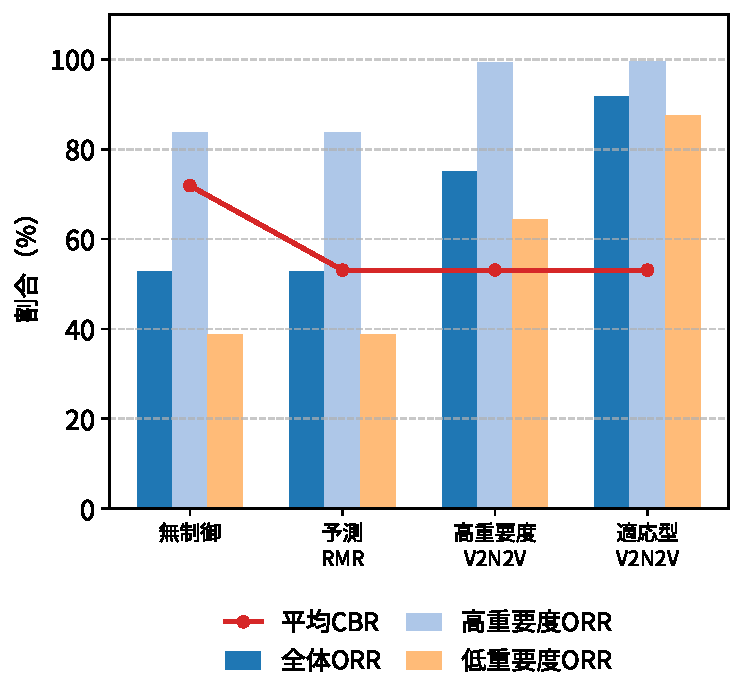
\includegraphics[width=\columnwidth]{result_graph.pdf}
\caption{各方式における周辺物標認識率（ORR）と平均CBRの比較結果}
\label{fig:result_graph}
\end{figure}

予測RMRは，無制御と同一の全体ORR（52.76\%）を維持したまま，チャネル混雑度（平均CBR）を0.719から0.531へと約26\%低減した．これは，上流交通流情報に基づく短期CBR予測が，NR-V2X sidelinkのチャネル負荷を抑制し，混雑時の通信余裕を確保する上で有効に機能したことを示している．

さらに提案方式である適応型V2N2Vは，高重要度ORRを99.54\%で維持しつつ，従来方式では38.85\%であった低重要度ORRを87.53\%まで向上し，全体ORRを91.67\%へと引き上げた．これは，高重要度情報の二重送信による高い到達性と，予測CBRに応じて低重要度情報も確率的にV2N2V経路で共有することで，V2V単独では未受信となる物標情報を補完できた結果である．
高重要度情報に限定してV2N2V経路を併用する方式と比較して，提案方式のV2N2V通信量は232.2\,MBから285.6\,MBへ増加したが，全体ORRを16.7ポイント，低重要度ORRを23.1ポイント向上させた．提案方式のV2N2V通信量は285.6\,MB/120\,s（約19.0\,Mbps）であり，高重要度V2N2V方式からの増加分は約3.6\,Mbpsであった．この追加負荷はNR-V2X sidelinkの局所CBRを増加させない一方，セルラ網側の収容性評価は今後の課題である．

\subsection{下流予測・先行通知の効果検証}
交通流の移動に基づく混雑先読みの有効性を分離評価するため，RSU区間ごとの基準CBRが変動する環境において，現在区間の実測CBRのみで制御する反応型方式と，下流区間のCBRを先行通知する先読み方式の比較を行った．

60秒間の平均ORRの差は反応型方式が82.40\%，先読み方式が82.64\%であったが，別途実施した固定CBR区間評価では，混雑区間に突入した直後である評価開始6秒時点において，全体ORRが87.22\%から90.95\%へと向上し，未受信率が11.00\%から5.99\%へ低下することを確認した．
また，移動高負荷区間の追従評価では，全6基中5基のRSUにおいて，実測CBRが制御閾値である0.6を超える3〜13秒前に，予測CBRが事前に閾値を超えることを確認した．この結果は，RSU間連携による下流混雑の先読み方式が，反応型方式の限界であった突入直後の通信バーストに伴う未受信の増加を抑制する先読みトリガーとして機能することを示した．

\section{まとめ}
本研究では，RSU間連携により交通流から下流区間のCBRを先読みし，物標の重要度に応じてV2VとV2N2Vのハイブリッド経路を動的に選択する経路制御方式を提案した．評価の結果，提案方式はNR-V2X sidelinkのチャネル負荷を抑制しつつ，V2N2V経路を併用することで全体のORRを91.67\%まで改善できることを示した．特に，混雑区間突入時における未受信率を低減させる先行通知の効果は，情報の鮮度が重要となる自動運転の安全協調認識において実用的な価値を持つことを確認した．

\begin{thebibliography}{9}
 \bibitem{yamasaki2023} 山崎 慎也, 「車両の走行環境を考慮した協調認識メッセージにおける冗長性緩和手法」, 同志社大学 修士論文, 2023.
\end{thebibliography}

\end{document}
